\chapter{Retrieval Augmented Generation (RAG) Dasar}
\label{chap:rag}

Masalah utama LLM adalah "Knowledge Cutoff". Jika Anda bertanya tentang berita pagi ini, ia tidak tahu.
RAG (Retrieval Augmented Generation) adalah solusi untuk masalah ini.

\section{Konsep Dasar RAG}

Secara sederhana, RAG adalah proses "menyontek" sebelum menjawab ujian.

\begin{enumerate}
    \item \textbf{Pertanyaan User:} "Siapa yang menang pertandingan bola semalam?"
    \item \textbf{Retrieval (Pencarian):} AI mencari artikel berita terbaru di database Anda.
    \item \textbf{Augmentation (Penambahan):} Artikel berita tersebut ditempelkan ke dalam prompt.
    \item \textbf{Generation (Generasi):} AI menjawab pertanyaan user \textit{berdasarkan} artikel yang ditemukan.
\end{enumerate}

\begin{center}
    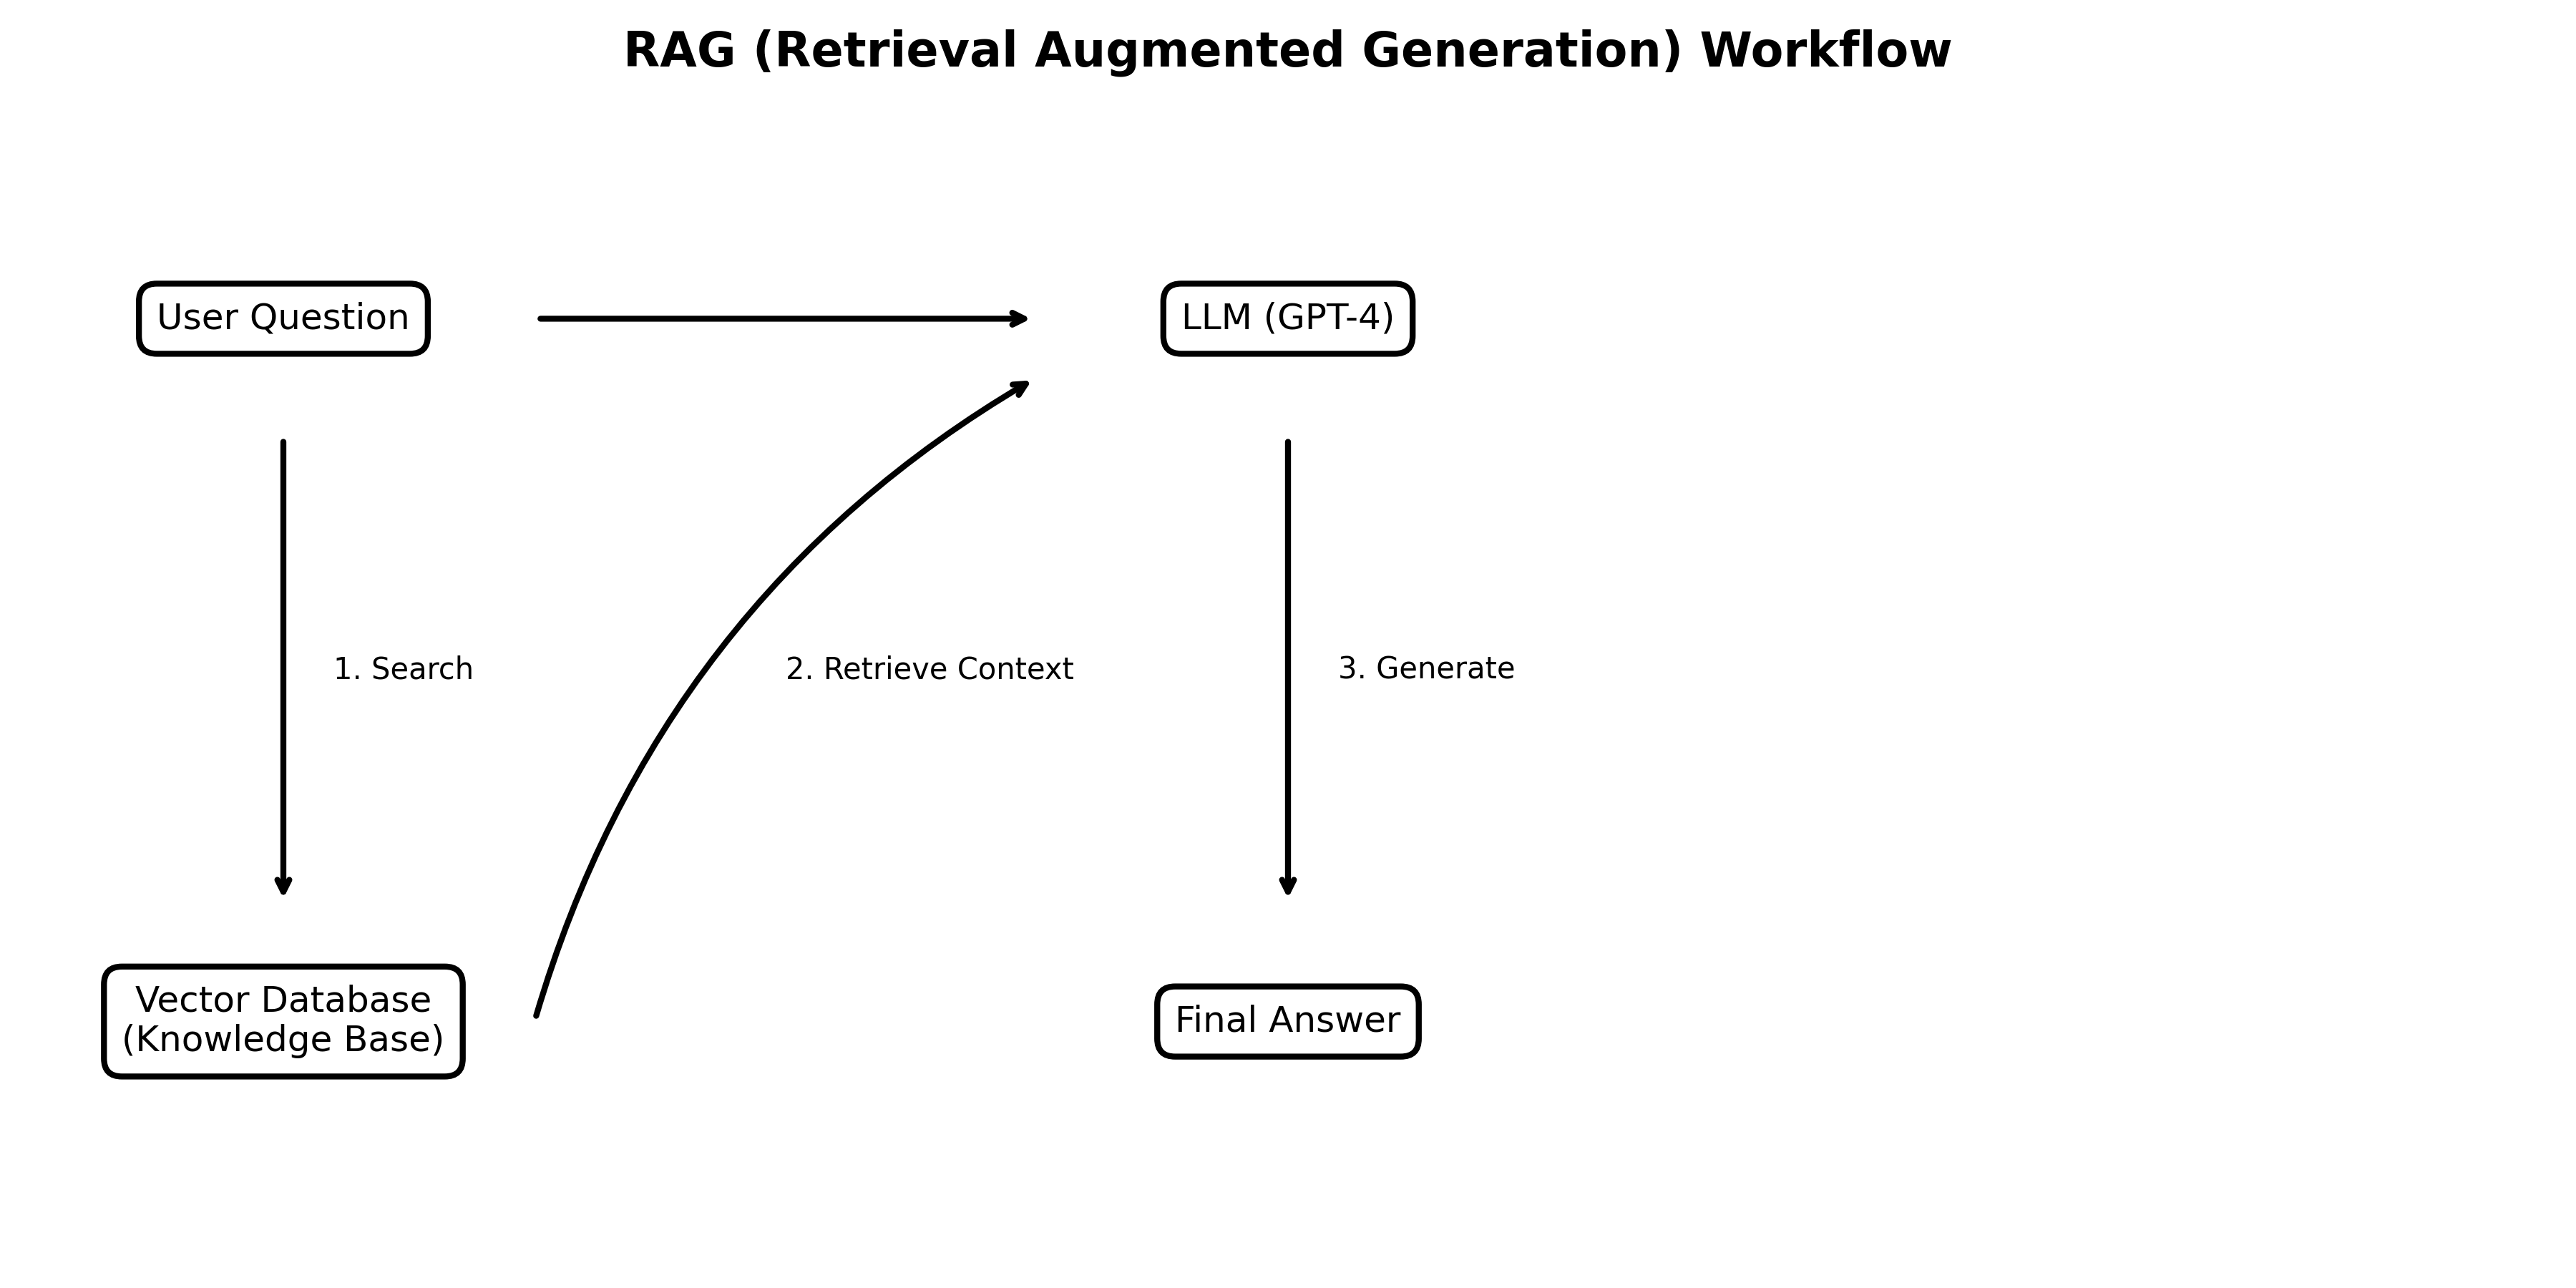
\includegraphics[width=\textwidth]{images/rag_diagram.png}
\end{center}

\section{Vector Embeddings: Bahasa Mesin}

Bagaimana komputer tahu bahwa kata "Kucing" mirip dengan "Meong"?

Jawabannya: **Vector Embeddings**.

Setiap kata atau kalimat diubah menjadi daftar angka panjang (misal 1536 dimensi untuk OpenAI). Kata-kata dengan makna serupa akan memiliki angka yang mirip secara matematis.

\begin{itemize}
    \item Kucing $\approx$ [0.1, 0.9, -0.5]
    \item Meong $\approx$ [0.12, 0.88, -0.4]
    \item Pesawat $\approx$ [0.9, -0.2, 0.1] (Jauh berbeda)
\end{itemize}

\section{Membangun "Chat with your PDF" Sederhana}

Untuk membuat aplikasi RAG yang bisa membaca PDF Anda, kita butuh beberapa tahap:

\begin{enumerate}
    \item **Load PDF:** Menggunakan library `PyPDF2` atau `LangChain Document Loader`.
    \item **Chunking:** Memecah teks PDF menjadi potongan-potongan kecil (misal 500 kata per chunk).
    \item **Embedding:** Mengirim setiap chunk ke OpenAI Embeddings API untuk mendapatkan vector-nya.
    \item **Store:** Menyimpan vector tersebut ke Vector Database (seperti Pinecone, ChromaDB, atau FAISS).
    \item **Retrieve:** Saat user bertanya, ubah pertanyaan user menjadi vector, lalu cari chunk yang paling mirip secara matematis (Cosine Similarity).
\end{enumerate}

\begin{tipbox}
\textbf{Mengapa Chunking Penting?}
Ingat Context Window? Kita tidak bisa memasukkan seluruh buku 500 halaman ke dalam prompt. Kita hanya mengambil bagian yang relevan saja.
\end{tipbox}

\section{Proyek Akhir Bagian III: Bot Customer Service}

Bayangkan Anda punya toko online. Anda ingin bot yang bisa menjawab pertanyaan tentang kebijakan pengembalian barang.

\textbf{Tanpa RAG:}
User: "Bisa retur barang rusak?"
AI: "Tergantung kebijakan toko Anda." (Jawaban umum dan tidak berguna).

\textbf{Dengan RAG:}
\begin{enumerate}
    \item Anda mengupload dokumen \texttt{kebijakan\_retur.txt} ke sistem RAG.
    \item User: "Bisa retur barang rusak?"
    \item RAG mencari di dokumen: menemukan kalimat "Barang rusak dapat diretur dalam 7 hari".
    \item Prompt ke AI: "Berdasarkan dokumen ini: 'Barang rusak dapat diretur dalam 7 hari', jawab pertanyaan user: 'Bisa retur barang rusak?'"
    \item AI: "Ya, Anda bisa meretur barang rusak dalam waktu 7 hari setelah pembelian." (Jawaban spesifik dan akurat).
\end{enumerate}
